\subsection{Board Page}

A board page is a page created under a workspace to organize tasks. On a board page, users can keep track of information
about projects and workflows, which helps you collaborate with your colleagues.\\

Once users have selected a workspace, they can create different board pages in the workspace A workspace can have multiple
boards at the same time. Click on one of them to go to the board page.\\

On board page users can create lists in their boards. Lists take cards, or specific tasks, and organize them by their
various stages of progress. Lists can be used to create a workflow. By clicking "Add another list", entering the list
title and clicking Add List, you can add your new list to your board page.\\

Users can create the required tasks to the list by adding cards.Just click “Add a card…” at the bottom of any list to create
a new card, and give it a name.Cards can be customized to hold a wide variety of useful information by clicking on them. By
clicking the Edit button, you can add, delete and change the activity, for example, modify the activity label, add or delete
members associated with the activity, add or delete time associated with the activity, and also move the card from start to
finish for each step of the process.
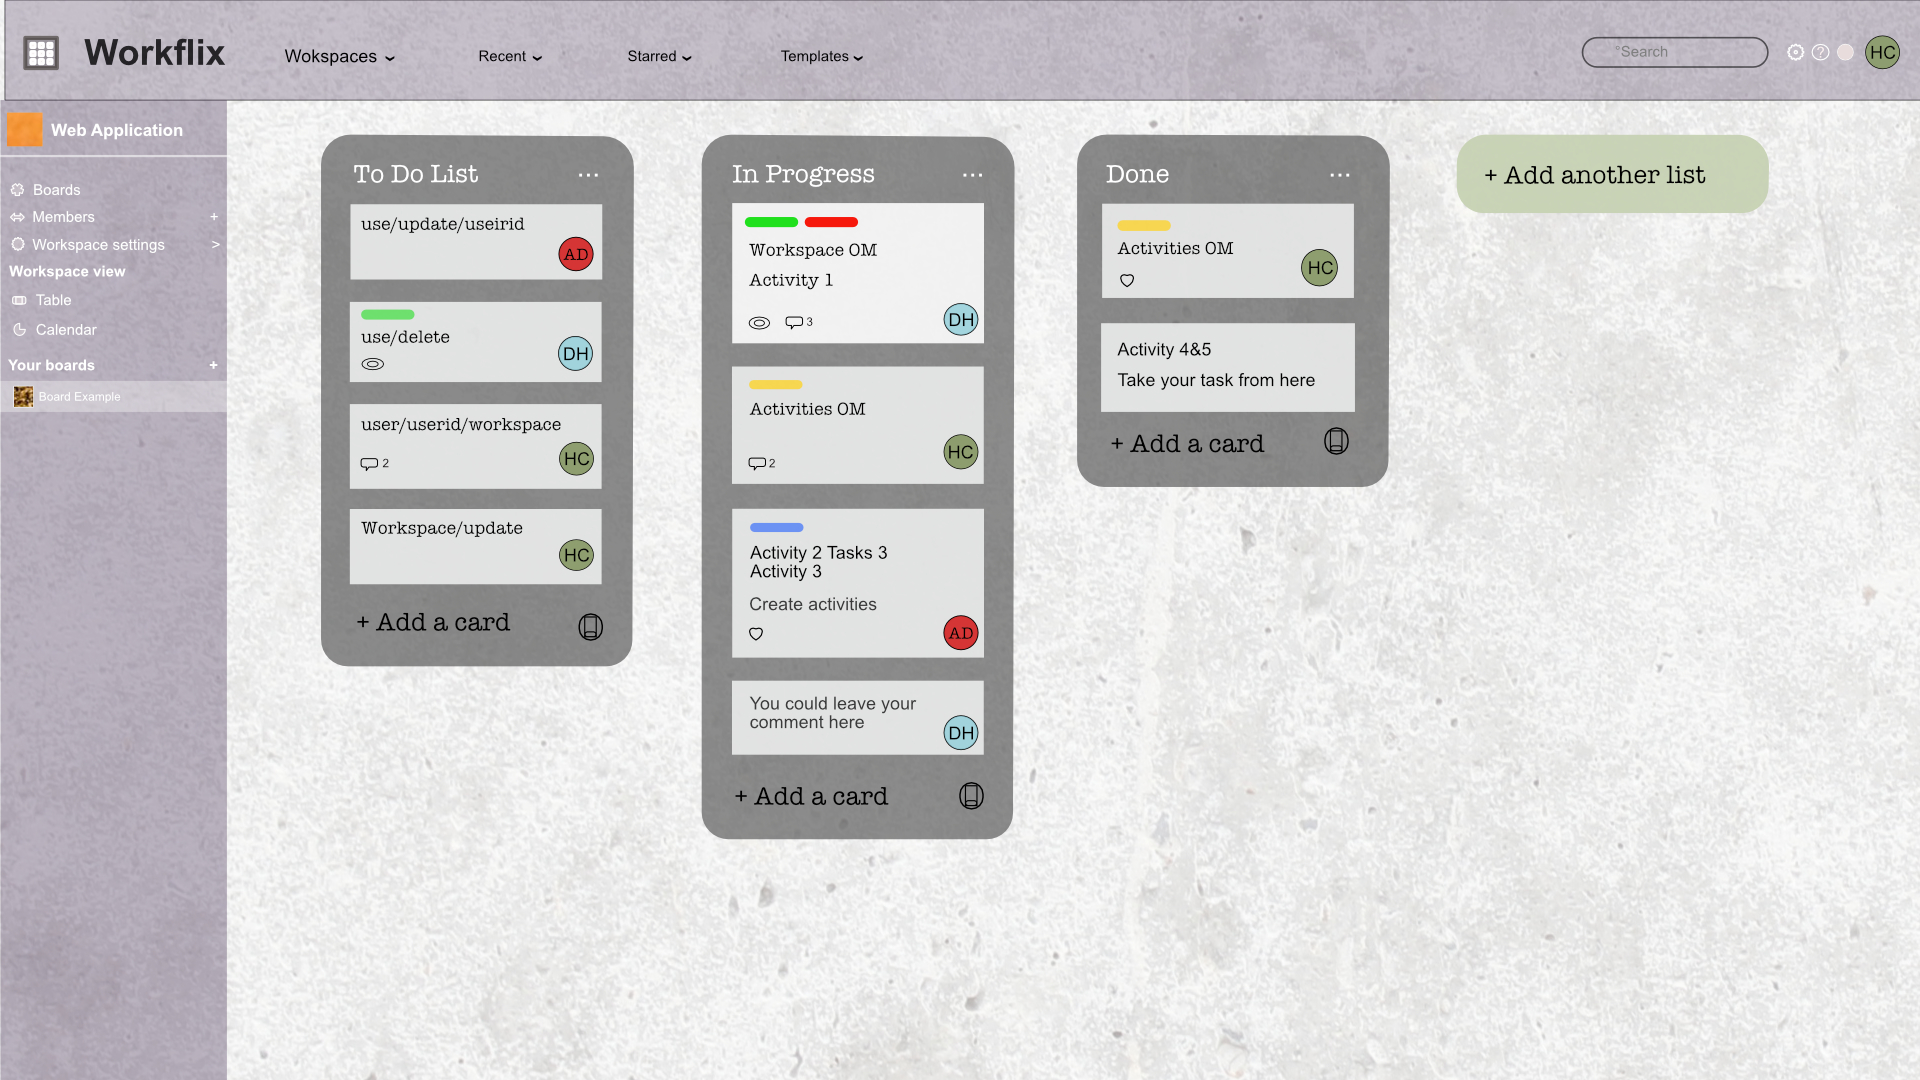
\includegraphics[width=\columnwidth]{images/Board.jpg}







